\documentclass[]{SRJcommon}
%%%%%%%%%%%%%%%%%%%%%%%%%%%%%%%%%%%
\title{One-dimensional computational transport}
\author{Seth R.~Johnson}
\date{2008/12/21}
%%%%%%%%%%%%%%%%%%%%%%%%%%%%%%%%%%%
\begin{document}
 \makeatletter
 \hypersetup{pdfauthor={\@author}, pdftitle={\@title}}
 \makeatother
%%%%%%%%%%%%%%%%%%%%%%%%%%%%%%%%%%%%%%%%%%%%%%%%%%%%%%%%%%%%%%%%%%%%%%%%%%%%%%%%
\maketitle
%%%%%%%%%%%%%%%%%%%%%%%%%%%%%%%%%%%%%%%%%%%%%%%%%%%%%%%%%%%%%%%%%%%%%%%%%%%%%%%%
\section{Exact one-group}
We consider the one-dimensional transport equation:
$$
\mu \oder{\psi}{x}( x, \mu) + \Sigma_t(x) \psi(x,\mu) 
= \int_{-1}^{1} \Sigma_{s}(\mu \mu') \psi(x,\mu')  \ud\mu' 
  + Q(x, \mu)
$$
or, writing the scattering in terms of Legendre polynomials, truncating to the
$L$th polynomial,
\begin{subequations}
  \label{eqs:exactwithbc}
\begin{equation}
\mu \pder{\psi}{x}( x, \mu) + \Sigma_t(x) \psi(x,\mu) 
= \sum_{l=0}^{L}  \frac{2l+1}{2} \Sigma_{sl}(x) P_{l}(\mu)
  \int_{-1}^{1} P_{l} (\mu') \psi(x,\mu')  \ud\mu' 
  + Q(x, \mu)\,,
  \label{eq:exact}
\end{equation}
for $0 \le x \le X$ and $-1 < \mu < 1$. This equation also has the boundary
conditions
\begin{align}
  \psi(0, \mu) &= \psi^L(\mu) \,, \quad 0 \le \mu < 1 
  \\
  \psi(X, \mu) &= \psi^R(\mu) \,, \quad -1 < \mu \le 0 \,.
\end{align}
\end{subequations}

%%%%%%%%%%%%%%%%%%%%%%%%%%%%%%%%%%%%%%%%%%%%%%%%%%%%%%%%%%%%%%%%%%%%%%%%%%%%%%%
\section{Discrete ordinates}
To formulate the discrete ordinates approximation, we let $\psi(\mu)$ only hold
on $N$ specific ordinate directions, each one with angle $\mu_n$ and weight
$w_n$. We always require $N$ to be even and that $\mu_n$ increase
with increasing $n$. The weights satisfy
$\sum_{n=1}^{N} w_n = 2$, analogous to how $\int_{-1}^{1} \ud \mu = 2$. 
The angular flux along each direction is $\psi(\mu_n) = \psi_n$.

Any integration over angle becomes a quadrature sum, so that
$$ \int_{-1}^{1} P_{l} (\mu') \psi(x,\mu')  \ud\mu'
\lra
\sum_{n'=1}^{N} w_{n'} P_{l} (\mu_{n'}) \psi_{n'}(x) \,.$$
The S$_\mathrm{N}$ equations are, modifying Eq.~\eqref{eq:exact},
\begin{equation}
\mu_n \oder{\psi_n}{x}(x) + \Sigma_t(x) \psi_n(x) 
= \sum_{l=0}^{L}  \frac{2l+1}{2} \Sigma_{sl}(x) P_{l}(\mu_n)
  \sum_{n'=1}^{N} w_{n'} P_{l} (\mu_{n'}) \psi_{n'}(x)
  + Q_n(x)
  \label{eq:sn}
\end{equation}
for $0 \le x \le X$ and $n=1,\ldots,N$.

An isotropic source should be 
\begin{equation}
Q_n(x) = \frac{1}{2} Q(x) \,.
  \label{eq:isotropicsource}
\end{equation}
Additionally, boundary conditions such as those in
Eqs.~\eqref{eqs:exactwithbc} are required. I have not yet looked into the
evaluation of discrete boundary conditions for an arbitrary incident flux, but
the reflecting boundary conditions $\psi(0, \mu) = \psi(0, -\mu)$ for $0 < \mu
< 1$ have their obvious counterpart in the \SN{} equations, for example:
$$ \psi_{n}(0) = \psi_{N + 1 - n}(0) \,, \quad N/2 + 1 < n < N  \,.$$

For vacuum boundaries, of course, $\psi_{n}(0) = 0$ for the incoming directions.
%%%%%%%%%%%%%%%%%%%%%%%%%%%%%%%%%%%%%%%%%%%%%%%%%%%%%%%%%%%%%%%%%%%%%%%%%%%%%%%
\subsection{The $k$-eigenvalue problem}
In the eigenvalue problem, the source $Q$ is replaced with a fission production
term, the product of the fission cross section, the number of neutrons emitted
per fission, and the scalar flux. (This gives the space-dependent production
rate of fission neutrons.)
It is scaled by $1/k$, a value which balances the production and loss
terms in the equation. Fission neutrons are always assumed to be emitted
isotropically, and since this is a one-group problem, $\chi = 1$. 
\begin{multline}
  \mu_n \oder{\psi_n}{x}(x) + \Sigma_t(x) \psi_n(x) 
\\
  = \sum_{l=0}^{L}  \frac{2l+1}{2} \Sigma_{sl}(x) P_{l}(\mu_n)
  \sum_{n'=1}^{N} w_{n'} P_{l} (\mu_{n'}) \psi_{n'}(x)
  + \frac{1}{k} \nu\Sigma_f(x) \sum_{n'=1}^{N} w_{n'} \psi_{n'}(x)
  \label{eq:fissionsn}
\end{multline}

In operator notation, Eq.~\eqref{eq:fissionsn} can be
written as
\begin{equation}
\op{L} \psi = \op{M} \op{S} \op{D} \psi +  \frac{1}{k} \op{F} \op{D} \psi \,,
  \label{eq:fissionoperator}
\end{equation}

where $\op{L}$ is the loss (leakage and absorption) operator; 
$\op{S}$ is the scattering operator, which works on the Legendre moments of
the angular flux; $\op{D}$ is the ``discrete-to-moments'' operator, which
integrates
the different moments of the discrete moments angular flux (mapping the
discretized angular flux to Legendre moments); $\op{M}$ is the
``moments-to-discrete'' operator; and $\op{F}$ is the
fission production operator. Moving the scattering operator to the left, and
inverting the transport operator,
$$ k \psi = (\op{L} - \op{M} \op{S} \op{D} )^{-1}  (\op{F} \op{D}) \psi \,,$$
is easily recognized as an eigenvalue problem.

[Note: in most computer programs, the full angular flux is never stored due to
memory requirements. Instead, only the scalar flux (and higher moments if
anisotropic scattering is present) is stored, using $\phi = \op{D} \psi$. Then,
when the transport sweep is performed, the flux moments are expanded via the
$\op{M}$ operator. Eq.~\eqref{eq:fissionoperator} is then
usually
\begin{align*}
\op{L} \psi &= \op{M} \op{S} \op{D} \psi +  \frac{1}{k} \op{F} [\op{D} \psi]
\\
( \op{L} -  \op{M} \op{S} \op{D} ) \psi &=  \frac{1}{k} \op{F} \phi
\\
k \psi &=  ( \op{L} - \op{M} \op{S} \op{D} ) ^{-1} \op{F} \phi
\\
k \op{D} \psi &= \op{D}  ( \op{L} - \op{M} \op{S} \op{D} ) ^{-1} \op{F} \phi
\\
k \phi &= \op{D} ( \op{L} - \op{M} \op{S} \op{D} ) ^{-1} \op{F} \phi
\end{align*}
See Ref.~\cite{War2004a} for more information on the detailed eigenvalue
problem.]

%%%%%%%%%%%%%%%%%%%%%%%%%%%%%%%%%%%%%%%%%%%%%%%%%%%%%%%%%%%%%%%%%%%%%%%%%%%%%%%
\subsection{Infinite medium}
The infinite-medium homogeneous \SN{} equations with an isotropic source are
$$\Sigma_t \psi_n 
= \sum_{l=0}^{L}  \frac{2l+1}{2} \Sigma_{sl} P_{l}(\mu_n)
  \sum_{n'=1}^{N} w_{n'} P_{l} (\mu_{n'}) \psi_{n'}
  + \frac{1}{2} Q_0 \,.$$

We multiply each equation by its corresponding weight, and add them all
together:
\begin{equation}
\Sigma_t \sum_{n=1}^{N} w_{n} \psi_{n} 
= \sum_{n=1}^{N} w_{n} \sum_{l=0}^{L}  \frac{2l+1}{2} \Sigma_{sl} P_{l}(\mu_n)
  \sum_{n'=1}^{N} w_{n'} P_{l} (\mu_{n'}) \psi_{n'}
  + \sum_{n=1}^{N} w_{n} \frac{1}{2} Q_0
  \label{eq:addedinf}
\end{equation}
The scalar flux is the zeroth Legendre moment of the equation ($P_l(\mu) = 1$),
so
$$ \phi(x) = \sum_{n=1}^{N} w_{n} \psi_{n}(x) \,.$$
Then, Eq.~\eqref{eq:addedinf} is:
$$ \Sigma_t [\phi] 
= \sum_{l=0}^{L}  \frac{2l+1}{2} \Sigma_{sl} \left[ \sum_{n=1}^{N} w_{n}
P_{l}(\mu_n) \right] \left[ \sum_{n'=1}^{N} w_{n'} P_{l} (\mu_{n'}) \psi_{n'}
\right] + \frac{1}{2} Q_0 [2] $$

If the Gauss-Legendre quadrature set is used (assuming a scattering order
smaller than the number of discrete ordinates used, i.e. $L < N-1$),
then the quadrature sum
produces the same result as the exact integral (see \cite[p.121]{Lew1984}):
$$ \sum_{n=1}^{N} w_{n} P_{l}(\mu_n) 
= \int_{-1}^{1} P_l(\mu) \ud \mu
= 2 \delta_{l0} \,.$$
In this case, the scattering term collapses and the equation becomes
\begin{align*}
  \Sigma_t \phi 
  &= \sum_{l=0}^{L}  \frac{2l+1}{2} \Sigma_{sl} \left[ 2 \delta_{l0} \right] \left[ \sum_{n'=1}^{N} w_{n'} P_{l} (\mu_{n'}) \psi_{n'}
\right] + Q_0
\\
  \Sigma_t \phi 
  &=  \frac{1}{2} \Sigma_{s0} (2) \left[ \sum_{n'=1}^{N} w_{n'} P_{0} (\mu_{n'}) \psi_{n'}
\right] + Q_0
\\
\Sigma_t \phi 
  &=  \Sigma_{s0} \phi + Q_0
\\
\phi 
&=  \frac{Q_0}{\Sigma_t - \Sigma_{s0}} \,.
\end{align*}
This is the well-known infinite medium result.
%%%%%%%%%%%%%%%%%%%%%%%%%%%%%%%%%%%%%%%%%%%%%%%%%%%%%%%%%%%%%%%%%%%%%%%%%%%%%%%%
\section{Spatial discretizations: finite difference}
We impose a spatial grid with $I+1$ points spanning $0 \le x \le X$. The
space-dependent cross sections and source are assumed to be piecewise-constant
inside the grid: for example, $\Sigma_t(x) = \Sigma_{t,i+1/2}$ for $x_{i} < x
< x_{i+1}$. The width of each spatial cell is $x_{i+1} - x_{i} \equiv
\Delta_i$. 

With finite difference equations, we integrate the \SN{} equations over each
spatial interval, operating on Eq.~\eqref{eq:sn} by $\int_{x_{i}}^{x_{i+1}}
(\cdot) \ud x$ for $i = 0,1,\ldots, I-1$.
This results in $I$ equations for each of the $N$ directions (so $I \cdot N$
total equations). Letting $\psi_{n,i} = \psi_n(x_i)$, we have
\begin{multline}
  \mu_n \left[ \psi_{n,i+1} - \psi_{n,i} \right] + \Sigma_{t,i+1/2}
  \int_{x_{i}}^{x_{i+1}} \psi_n(x) \ud x
\\
= \sum_{l=0}^{L}  \frac{2l+1}{2} \Sigma_{sl,i+1/2} P_{l}(\mu_n)
 \sum_{n'=1}^{N} w_{n'} P_{l} (\mu_{n'}) \int_{x_{i}}^{x_{i+1}} \psi_{n'}(x) \ud x
  + Q_{n,i+1/2} \int_{x_{i}}^{x_{i+1}} \ud x
  \label{eq:finitediff}
\end{multline}
From this
point, we make the substitution $X_{i+1/2} \to X_{i}$ for brevity, keeping in
mind that the cross section or source for index $i$ refers to the cell between
$x_i$ and $x_{i+1}$.

The \emph{diamond difference} discretization essentially assumes that the
``cell-averaged flux'' is the average of the two cell-edge fluxes, so the
essential approximation is that
\begin{equation}
  \frac{1}{x_{i+1} - x_{i}} \int_{x_{i}}^{x_{i+1}} \psi_{n}(x) \ud x
 = \frac{1}{\Delta_i} \int_{x_{i}}^{x_{i+1}} \psi_{n}(x) \ud x
\approx  \frac{1}{\Delta_i} \frac{\psi_{n,i+1} + \psi_{n,i}}{2} 
\,.
  \label{eq:diamondapprox}
\end{equation}
This is essentially the same as ``Crank-Nicholson differencing,'' so we expect
the diamond difference method to have $O(\Delta^2)$ global error but to be
potentially subject to oscillations.

We have a total of $N\cdot(I+1)$ unknowns: the angular flux in every
direction $N$ on every grid point. The missing equations are resolved by the
boundary condition: on the left boundary ($i=0$) the angular flux $\phi_{n,0}$
for incoming directions ($\mu_n > 0$) must be specified, and likewise on the
right boundary ($i=I$) the angular flux $\phi_{n,I}$ must be specified
for directions with $\mu_n < 0$.

For isotropic scattering, Eq.~\eqref{eq:finitediff} has $L=0$, and simplifies to
$$
 \mu_n \left[ \psi_{n,i+1} - \psi_{n,i} \right] + \Sigma_{t,i}
  \int_{x_{i}}^{x_{i+1}} \psi_n(x) \ud x
= \frac{1}{2} \Sigma_{s0,i} 
 \sum_{n'=1}^{N} w_{n'}  \int_{x_{i}}^{x_{i+1}} \psi_{n'}(x) \ud x
  + Q_{n,i}  \Delta_i
$$
Substituting Eq.~\eqref{eq:diamondapprox} and dividing by $\Delta_i$, we have equations for
$i=0,\ldots,I-1$ and $n=1,\ldots,N$:
\begin{equation}
  \frac{\mu_n}{\Delta_i}  \left[ \psi_{n,i+1} - \psi_{n,i} \right]
+ \Sigma_{t,i}  \left[ \frac{\psi_{n,i+1} + \psi_{n,i}}{2} \right]
=
\frac{1}{2} \Sigma_{s0,i}
\sum_{n'=1}^{N} w_{n'} \left[ \frac{\psi_{n',i+1} + \psi_{n',i}}{2} \right]
  + Q_{n,i} \,.
  \label{eq:ddfinal}
\end{equation}

%%%%%%%%%%%%%%%%%%%%%%%%%%%%%%%%%%%%%%%%%%%%%%%%%%%%%%%%%%%%%%%%%%%%%%%%%%%%%%%%
\subsection{Direct matrix representation}
The Eq.~\eqref{eq:ddfinal} can be implemented directly in a sparse matrix
formulation along with the boundary conditions. (See the MATLAB
code and Fig.~\ref{fig:transportmatrix}.)
They form the transport matrix, which is inverted and applied to a source
vector to solve the transport problem.

\begin{figure}[htb]
  \centering
  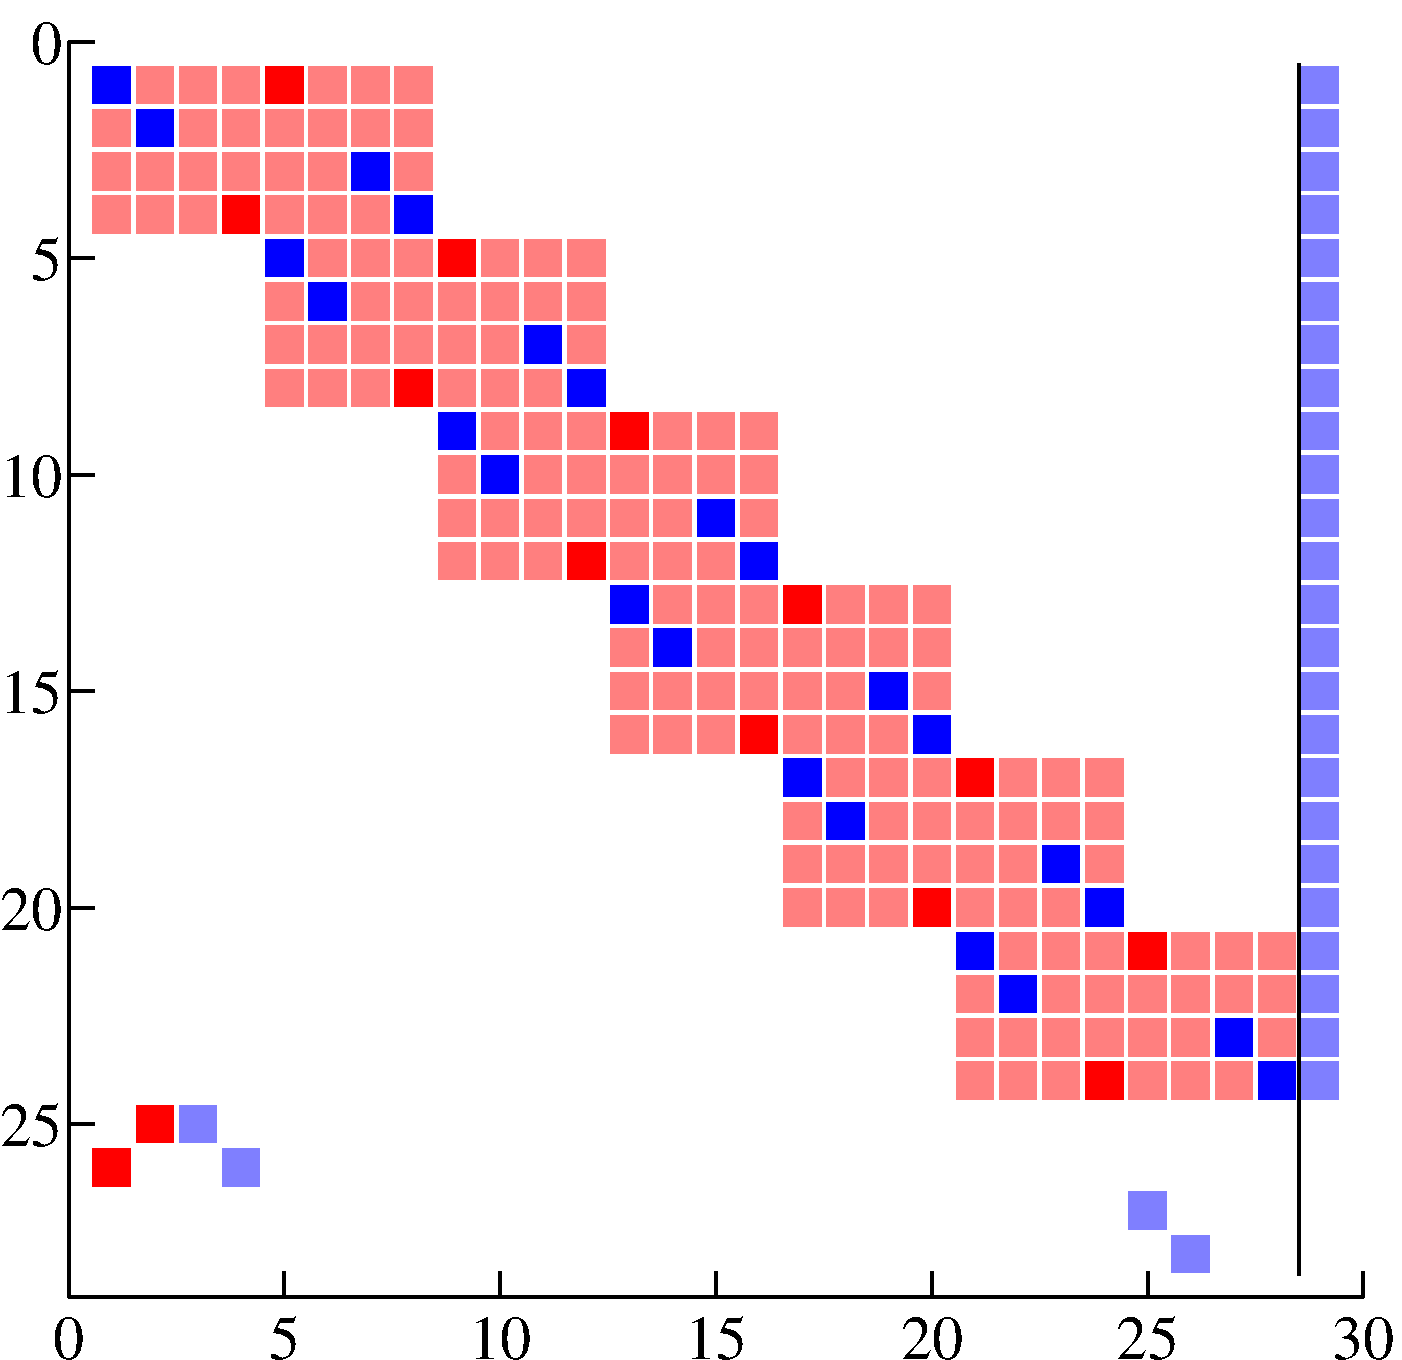
\includegraphics[width=3.5in]{matrix}
  \caption{This is the diamond difference, discrete ordinate transport matrix
  $\op{L} - \op{M} \op{S} \op{D}$
  for $N=4$ and $I=6$, along with the source vector, which is the rightmost
  column. Blue entries are positive (darker blue is more
  positive), and red entries are negative (darker red is more negative). The
  first 24 rows correspond to Eq.~\eqref{eq:ddfinal}, the next two are for a
  reflecting boundary condition on the left, and the final two are for a vacuum
  boundary on the right.}
  \label{fig:transportmatrix}
\end{figure}

The source vector will have $I\cdot N$ terms comprising the source for
each angle $n$ inside each cell $i$, and it will also have $N$ terms for the
boundary conditions.
The boundary condition equation for a vacuum boundary on the left side will be:
$$ \psi_{0,n} = 0 \,, \quad n= N/2 + 1, \ldots, N \,.$$
For a reflecting condition on the right side, it will be:
$$ \psi_{I,n} - \psi_{I,N+1-n} = 0 \,.$$
Unless there is a static, known incident flux on the boundary, the additional
boundary sources on the source vector will therefore be zero.
%%%%%%%%%%%%%%%%%%%%%%%%%%%%%%%%%%%%%%%%%%%%%%%%%%%%%%%%%%%%%%%%%%%%%%%%%%%%%%%%
\subsection{Transport sweeps}
Most traditional codes are based on a method called \emph{source iteration}
(SI). In this method, the inscattering term of Eq.~\eqref{eq:exact},
or the ``scattering source,'' is based on the previous
iteration's flux $\phi^{(\ell)}(x,\mu)$ and lumped with the
extraneous source $Q(x,\mu)$ to form $\tilde{Q}^{(\ell)}(x,\mu)$, the total
source for the new iteration.

One of the distinct advantages of a finite difference formulation of a
differential equation is that, along each direction $\mu_n$, the SI method
updates the next spatial point's flux $\psi_{n,i}^{(\ell+1)}$ using only the
flux at the previous point $\psi_{n,i-1}^{(\ell+1)}$ and the ``known'' source
$\tilde{Q}_{i}^{(\ell)}$. To show this, we write Eq.~\eqref{eq:ddfinal} in
terms of the total source and with iteration indices:
\begin{subequations}
  \label{eq:dditeration}
\begin{equation}
  \frac{\mu_n}{\Delta_i}  \left[ \psi_{n,i+1}^{(\ell+1)} - \psi_{n,i}^{(\ell+1)} \right]
+ \Sigma_{t,i} \left[ \frac{\psi_{n,i+1}^{(\ell+1)} + \psi_{n,i}^{(\ell+1)}}{2} \right]
= \tilde{Q}_{i}^{(\ell)}
  \label{eq:ddsweep}
\end{equation}
and (with isotropic scattering)
\begin{equation}
 \tilde{Q}_{i}^{(\ell)}
 =
\frac{1}{2} \Sigma_{s0,i} 
\left[ \frac{\phi_{i+1}^{(\ell)} + \phi_{i}^{(\ell)}}{2} \right]
+ \frac{1}{2} Q_{i}  \,,
  \label{eq:ddsource}
\end{equation}
where
\begin{equation}
  \phi_{i}^{(\ell)} = \sum_{n'=1}^{N} w_{n'} \psi_{n',i+1}^{(\ell)}
  \label{eq:phi}
\end{equation}
\end{subequations}
is used to reduce the storage requirements between iterations. [If anisotropic
scattering is used, higher moments of the flux must also be stored, and then
the total source $\tilde{Q}_{i}^{(\ell)}$ will be anisotropic as well.]

Solving Eq.~\eqref{eq:ddsweep} for $\psi_{n,i+1}^{(\ell+1)}$,
\begin{align*}
%  \left[  \frac{\mu_n}{\Delta_i} + \frac{\Sigma_{t,i}}{2} \right]
%    \psi_{n,i+1}^{(\ell+1)}
% + \left[ - \frac{\mu_n}{\Delta_i} + \frac{\Sigma_{t,i}}{2} \right]
%    \psi_{n,i}^{(\ell+1)}
%&= \tilde{Q}_{i}^{(\ell)}
%\\
%\psi_{n,i+1}^{(\ell+1)} + 
%  &= \left( \frac{\mu_n}{\Delta_i} + \frac{\Sigma_{t,i}}{2} \right)^{-1}
%\left[ \tilde{Q}_{i}^{(\ell)} - \left( - \frac{\mu_n}{\Delta_i} +
%\frac{\Sigma_{t,i}}{2} \right) \psi_{n,i}^{(\ell+1)} \right]
%\\
\psi_{n,i+1}^{(\ell+1)}
  &= \left( \frac{\mu_n}{\Delta_i} + \frac{\Sigma_{t,i}}{2} \right)^{-1}
\left[ \left( \frac{\mu_n}{\Delta_i} -
\frac{\Sigma_{t,i}}{2} \right) \psi_{n,i}^{(\ell+1)}
+ \tilde{Q}_{i}^{(\ell)} \right] \,.
\end{align*}
So, the angular flux in one direction for a new iteration depends only on the
flux at the previous grid point in the new iteration and on the total source
from the previous iteration. This process of updating the new angular flux
iterate is called a ``sweep.''

Boundary conditions are applied at the beginning the sweep. If the sweep starts
from a vacuum boundary, the starting flux is zero. If the sweep starts from a
reflecting boundary, it is advantageous to perform the sweep for the
angle opposite to the incoming reflected angle and then to use the ``outgoing''
angular flux that was just calculated.
%%%%%%%%%%%%%%%%%%%%%%%%%%%%%%%%%%%%%%%%%%%%%%%%%%%%%%%%%%%%%%%%%%%%%%%%%%%%%%%%
%%%%%%%%%%%%%%%%%%%%%%%%%%%%%%%%%%%%%%%%%%%%%%%%%%%%%%%%%%%%%%%%%%%%%%%%%%%%%%%%
\nocite{Lew1984}\nocite{Lar2007}
\bibliographystyle{siam}
\bibliography{references}
\end{document}
